\graphicspath{{figures/chapter1/}}
\onehalfspacing

\chapter{Introduction}\label{ch:introduction}

\vfill

\newthought{This chapter is based on:}

\noindent 

\begin{itemize}
    \item De Gaetani, C. I., Ioli, F., \& Pinto, L. (2021). Aerial and UAV Images for Photogrammetric Analysis of Belvedere Glacier Evolution in the Period 1977–2019. Remote Sensing, 13(18), 3787. \url{https://doi.org/10.3390/rs13183787}
    \item Ioli, F., Bianchi, A., Cina, A., De Michele, C., Maschio, P., Passoni, D., \& Pinto, L. (2021). Mid-Term Monitoring of Glacier’s Variations with UAVs: The Example of the Belvedere Glacier. Remote Sensing, 14(1), 28. \url{https://doi.org/10.3390/rs14010028}
    \item Ioli, F., Dematteis, N., Giordan, D., Nex, F., Pinto, L. (2024). Deep Learning Low-cost Photogrammetry for 4D Short-term Glacier Dynamics Monitoring. \textit{PFG}. \url{https://doi.org/10.1007/s41064-023-00272-w}
\end{itemize}

\newpage

\section{Motivation and relevance}

Glaciers all over the world are experiencing profound transformations due to the ongoing climate crisis~\citep{Oerlemans2005} and their sensitivity to temperature fluctuations renders them powerful indicators of global climate change~\citep{Barry2016}.
Alpine glaciers, situated in temperate zones, are particularly susceptible to rising temperatures. The accelerated rate of glacial retreat underscores the necessity for comprehensive monitoring programs~\citep{Zemp2006,Sommer2020}. 
Therefore, they are often considered as a proxy for climate change evaluation.
Projections point out that the European Alps may lose more than 60\% of ice volume by the end of the century under the RCP2.6 scenario, whereas a larger amount of ice loss is expected under worse scenarios~\citep{Zekollari2019}.

However, mountain glaciers are a critical component of the local economy regarding freshwater supply, hydroelectric production, and tourist activities.
In particular, glaciers serve as critical as crucial freshwater reservoirs and their undergoing transformation is likely to have severe consequences for the future water availability~\citep{Barnett2005, hock2005}. 
Additionally, glacier melting and retreat are triggering several glaciological processes, e.g., ice break-off, glacier outburst, snow/ice avalanches, and gravitational slope stability processes, such as rockfalls and collapses, and debris flow, which can threaten the population, urban areas or infrastructure of the nearby areas~\citep{Kaab2004, Deline2015, Giordan2020}.
In the European Alps, the number of mass movements and hazardous events in high-elevations environments has experienced an increase in the past decade due to climate change~\citep{chiarle2023, Nigrelli2024}.

A relevant and tragic example was the collapse of a section of the Marmolada Glacier (Dolomites, Italy), which occurred on 3 July 2022 at 13:43:20 CEST\footnote{\url{https://www.theguardian.com/world/2022/jul/03/deaths-glacier-breaks-marmolada-mountain-italy}}. 
The collapse caused an ice avalanche that killed 11 mountaineers trying to reach the Marmolada summit and injured 7~\citep{Olivieri2023, Bondesan2023}.
The collapse occurred on the northern slope of the glacier at an elevation of \SI{3213}{\masl} and involved a volume of \SI{\sim 96000}{\cubic\meter}~\citep{Olivieri2023}.
The detachment was caused by a failure along a median crevasse, partially filled by meltwater due to highly anomalous temperatures, that reached \SI{10.7}{\degree\celsius} at the time of the event.
The sudden glacier collapse was probably induced by a combination of hydraulic jacking and pressure within a thin layer of basal till~\citep{Bondesan2023}.

Just one year after the Marmolada collapse, another relevant event slope instability event was registered in the Austrian state of Tyrol, close to the Italian border. 
On 11 June 2023, a big portion of the summit of Fluchthorn, a nearly \SI{3400}{\masl} has collapsed sending more than \SI{100000}{\cubic\meter} of rock crashing into the valley below and triggering mudslides\footnote{\mbox{\url{https://edition.cnn.com/2023/06/14/europe/austrian-mountain-fluchthorn-rockslide-climate-intl/index.html}}}.
This event was likely related to the thawing permafrost due to the high temperatures of that period\footnote{\url{https://blogs.agu.org/landslideblog/2023/06/12/fluchthorn-1/}}.

On 30 August 2023, a large debris flow occurred at the Belvedere Glacier (Anzasca Valley, Italian Alps)\footnote{\url{https://www.regione.piemonte.it/web/temi/protezione-civile-difesa-suolo-opere-pubbliche/protezione-civile/sorvolo-ghiacciai-monte-rosa-07092023}}.
The debris flow was triggered at the beginning of the steep Castelfranco gully, located at approximately \SI{3600}{\masl} on the streamwise-left side of the Belvedere Glacier north-west lobe.
During the event, a volume of \SI{\sim 200000}{\cubic\meter} was accumulated on top of the Belvedere Glacier and obstructed the sinkhole that allowed the Castelfranco stream to flow below the ice sheet. 
This caused the water to stream on top of the glacier, carving deep grooves on top of the Belvedere Glacier. 
A large portion of the debris was transported towards the valley and the municipality of Macugnaga by the river Anza and cumulated in the riverbed.
A previous event with similar characteristics but significantly smaller dimensions occurred in 2008 and was documented by \cite{Mortara2009_ghiacciaoBelvedere}, who reported an estimation of the cumulated debris volume of a few thousand cubic meters.

In this context, long-term monitoring of glaciers and related glaciological processes assumes a crucial significance.
To achieve a thorough understanding of these complex systems, systematic observations are essential~\citep{Kaab2005}.
A particular focus is usually placed on monitoring surface kinematics, as these can potentially offer early warning signs of impending instability or collapse events~\citep{Faillettaz2015}.
Nevertheless, monitoring glaciers in remote areas and inaccessible terrains often presents logistical and safety challenges.
Therefore, remote sensing techniques are widely used as they allow for observing glacial processes with minimal risk for scientists and technicians. 

In the past 30 years, the availability of free and commercial satellite imagery, with various spatial, temporal, and radiometric resolutions, has widely enlarged the possibility of sensing remote areas.
The literature for satellite-based global or regional mapping of glaciers is nowadays extremely wide and covers different aspects of glacier monitoring \citep{Paul2007}. 
This includes glacier outline mapping from optical imagery (\textcolor{red}{REF}) or from combinations of different bands~\citep{Winsvold2016}, such as Red and SWIR bands or the near-infrared and SWIR (short-wave infrared band)~\citep{Paul_2002} or the normalized difference snow index (NDSI)~\citep{Hall1995}.
Planimetric glacier displacements and flow velocity are often derived from ortho-projected products with digital image correlation (DIC) techniques~\citep{Scambos1992, Kaab2005, Scherler2008, altena_kaab_2020}. 
Satellite remote sensing has been used also for estimating mass balances~\citep{Bamber2007, Berthier2016, Rabatel2017, Berthier2023}.
\textcolor{red}{(SAR and passive satellites?)}
% \textcolor{red}{Satellite SAR data \citep{Strozzi2020, Fang2016, Winsvold2018}.}

Although satellite remote sensing is essential for large-scale regional or even global glacier monitoring, most of the free solutions offer limited spatial and temporal resolution, which hinders the ability to sense small alpine glaciers and capture short-term glacier dynamics. 

\textcolor{red}{...Conclude this intro su satellite with high-res optical sats...}

\textcolor{red}{...Part on aerial photogrammetry for mid-to-large scale and long-term freq...}

In the past decade, Unmanned Aerial Vehicles (UAVs) have undergone rapid technological advancements and cost reductions,
making them indispensable tools for environmental monitoring. 
Coupled with modern Structure-from-Motion (SfM) \citep{Westoby2012} and Multi-View Stereo (MVS) \citep{Seitz2006} algorithms, 
images captured by UAV-mounted cameras enable the creation of high-resolution 3D point clouds, Digital Surface Models (DSMs),
and orthophotos. 
Their applications in environmental studies are extensive, including geomorphology modelling~\citep{Cook2017, James2017_3duncertainty}, 
river flow velocity and discharge estimation~\citep{Detert2017,Ioli2020}, 
snow volume calculation~\citep{DeMichele2016, Buhler2016, Avanzi2018},
dam sediment volume evaluation~\citep{Pagliari2016}, glaciers \citep{Immerzeel2014, Chudley2019, Groos2019}, 
periglacial morphology \citep{Sledz2021}.

Several examples of UAV and photogrammetry applications for cryosphere monitoring can be found in the literature~\citep{Bhardwaj2016, Gaffey2020}.
For instance, \cite{Whitehead2013} employed fixed-wing and helicopter-based UAVs equipped with low-cost cameras to generate orthophotos 
and DSMs of the Fountain Glacier in the Canadian Arctic. 
Similarly,~\cite{Immerzeel2014} and \cite{kraaijenbrink2016} leveraged fixed-wing UAVs for evaluating seasonal surface velocities of the debris-covered
Lirung Glacier in Nepal. 
\cite{Gindraux2017} further investigated the impact of Ground Control Point (GCP) quantity and distribution on the accuracy of UAV-derived glacier DSMs 
and she proposed a technique based on the joint usage of Digital Image Correlation (DIC) on both DSMs and orthophotos to derive glacier kinematics.
The growing body of recent work highlights the potential of UAVs and low-cost photogrammetry to efficiently monitor small and mid-scale 
glaciers with high spatial resolution, as they enable comprehensive reconstruction of glacier morphology while minimizing in-situ operations and
costs \citep{Benoit2019, Chudley2019, Jouvet2020, Cao2021, Lamsters2022, belloni2023}.
Moreover, studies like \cite{ioli2021mid} demonstrate the feasibility of using UAVs for mid-term (i.e., ten-year span) glacier monitoring with 
very high spatial resolution and annual temporal frequency.
 
\textcolor{red}{... Part on in-situ monitoring for high spatial res and frequency...}
While UAVs vastly improve spatial resolution, they might not fully replace in-situ monitoring for tasks requiring high temporal frequency 
(e.g., continuous measurements)....


% Over the years, various remote sensing approaches have been utilized to
% capture the glacier dynamics and evolution. These approaches include satellite-based
% sensing~\citep{altena_kaab_2020,Scherler2008}, satellite Synthetic Aperture Radar
% (SAR)~\citep{Strozzi2020}, 3D photogrammetric reconstruction from
% UAVs~\citep{Chudley2019,Ioli2022},
% aerial platforms~\citep{Degaetani2021} and optical high-resolution
% satellite~\citep{Tonolo2020},
% ground-based monoscopic or stereoscopic time-lapse
% cameras~\citep{Messerli2015,Schwalbe2017,Hendrickx2022},
% ground-based SAR~\citep{Dematteis2018,Noferini2009},
% aerial and UAV laser scanner \citep{Hartl2023} or Terrestrial Laser Scanners
% (TLS)~\citep{Hendrickx2022,Voordendag2023}.

% Permanent terrestrial SAR and TLS have gained significant attention for short-term
% monitoring.
% SAR, in particular, offers all-weather and day-and-night imaging, making it suitable for
% real-time monitoring and early-warning systems~\citep{Dematteis2021,Noferini2009}.
% However, both ground-based SAR and permanent TLS are expensive, requires complex
% logistics.
% These limitations prevent their applications in distributed sites at regional scale, but
% their usage may be limited to investigate hazardous locations.

% Fixed time-lapse cameras offer an affordable alternative to terrestrial SAR and TLS for
% gathering qualitative and quantitative information on glacier
% dynamics~\citep{Giordan2016,James2016, Maas2006,Messerli2015}.
% Digital Image Correlation (DIC) can be used on sequences of images from terrestrial
% time-lapse cameras to estimate glacier surface velocity.
% Initially used in laboratory settings, DIC was first applied to glaciers
% by~\citet{Evans2000}. Subsequently, numerous studies employed this
% technique for measuring glacier kinematics
% \citep{ahn_box_2010,Giordan2016,Hadhri2019,James2016,Messerli2015}.
% However, external Digital Surface Models (DSMs) are required to convert 2D pixel
% displacements obtained by DIC into 3D displacement vectors.

% \cite{Paul2015, KaabFunk1999}

\section{Objectives}

\section{The Belvedere Glacier}\label{sec:1:belvedereglacier}

The Belvedere Glacier (Randolph Glacier Inventory code RGI60--11.02858) is an alpine
glacier in Valle Anzasca (Italy), on the east side of the Monte Rosa Massif (N
\ang{45;58} E \ang{7;55}) (\figref{fig:1:studyarea}).
The lower part of the Belvedere Glacier is a temperate debris-covered glacier, that
covers an area of
\SI{\sim1.8}{\kilo\meter\squared} and extends from an altitude of \SI{\sim2250}{\masl} to
\SI{\sim1800}{\masl}.
This region is characterized by a gentle slope, and it is fed by ice falls and snow
avalanches coming from the Monte Rosa East Face \citep{Haeberli2002}. In its low-relief
sector, the Belvedere Glacier splits into two lobes, reaching \SI{\sim1800}{\masl}.
The northern lobe, in particular, ends with a prominent ice cliff, from which the River
Anza springs.

Similarly to Miage glacier (Monte Bianco, Valle d’Aosta), the Belvedere Glacier is almost
completely covered by rocks and boulders with dimensions ranging from few decimetres to
some meters, which makes it a \textit{black glaciers}.
Due to the global warming trend, the~number of black glaciers along the Italian Alps is
rising~\citep{Diolaiuti2003}.
Up to the beginning of the century, the~debris cover helped to compensate the effect of
the increased temperature, establishing a negative feedback in the temperature-ablation
relationship~\citep{Roethlisberger1985,Diolaiuti2003}.
However, in~recent years, the~debris cover protection has not been sufficient to limit
the glacier~retreat.

\begin{figure}
    \centering
    \subcaptionbox{\label{fig:1:studyarea:map}}{
        \includegraphics[height=5cm]{belvedere_location.png}
    }
    \subcaptionbox{\label{fig:1:studyarea:pic}}{
        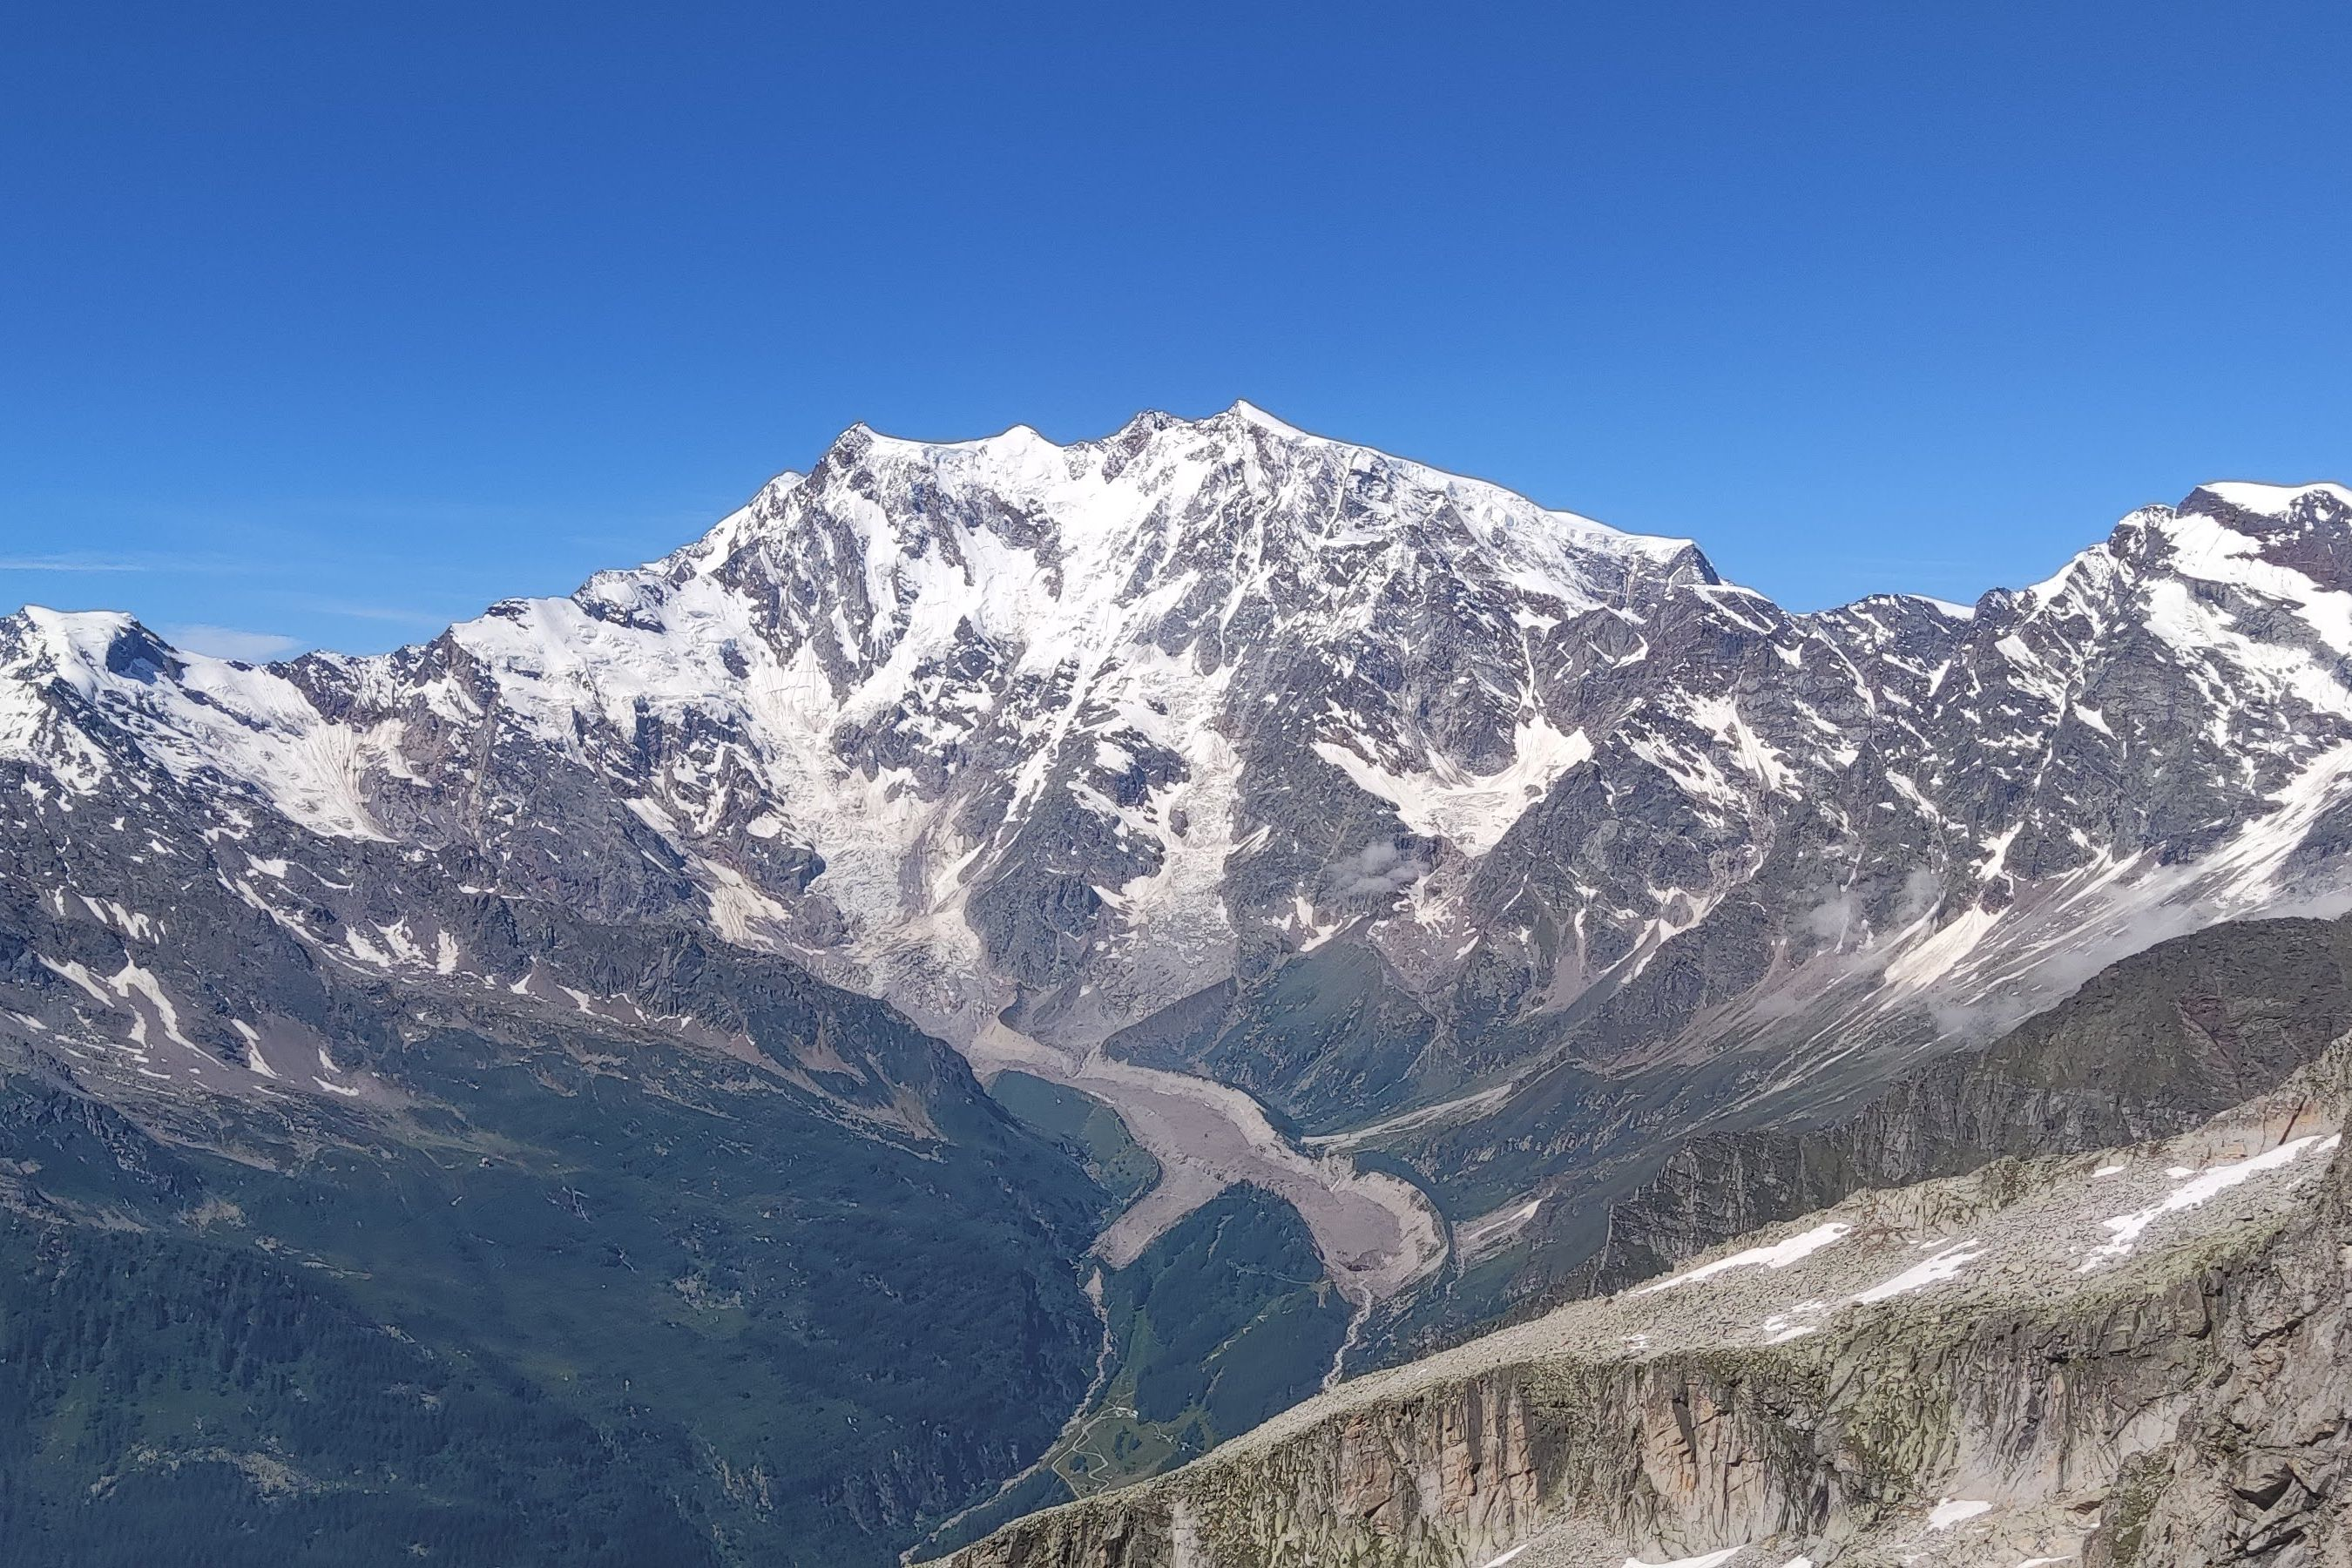
\includegraphics[height=5cm]{belvedere_pic.jpg}
    }
    \caption{(a) Location of Belvedere Glacier, base map (source: Swisstopo
        www.geo.admin.ch); (b) Picture of \textcolor{red}{...}}
    \label{fig:1:studyarea}
\end{figure}

In the past, several hazardous events originated by the Belvedere Glacier, such as floods
and slope instability, threatened the nearby village of Macugnaga and the Zamboni Zappa
Hut, at 2070 m a.s.l. \citep{Kaab2004}.
At the beginning of the 21st century, the Belvedere Glacier was characterized by a
particular surge-type dynamics  \citep{Haeberli2002}.
During the late 1990s, the~surface speeds of the whole glacier were ranging between
\SIlist{30;45}{\meter\per\year}~\citep{Roethlisberger1985, Kaab2005}.
During 2000--2001 an accelerated flow in the Monte-Rosa Glacier produced a wave of
compression-decompression stresses and strains in the Belvedere Glacier.
Surface velocities soared: values up to \SI{200}{\meter\per\year} were observed
photogrammetrically during autumn 2001~\citep{Kaab2004}.
The ice thickness increased more than~\SI{20}{\meter} and the wave travelled downwards,
creating a depression area in the accumulation zone, that was filled by a super-glacial
lake, the~Lago Effimero~\citep{Haeberli2002, Mortara2009}.


During spring 2002, the large depression at the foot of the Monte Rosa east face caused by the 
surge-type movement was temporarily filled by a lake with a volume of \SI{3e6}{\cubic\meter}, 
the socalled \textit{Lago Effimero} (\textit{short-lived lake}).
Recognizing the potential danger of an outburst flood, the Italian Civil Defense Department rapidly 
implemented emergency measures, including evacuating parts of Macugnaga village, installing automatic 
alarm systems and pumps, and initiating detailed scientific investigations. 
Reduced meltwater input in July 2002, combined with natural subglacial drainage, stabilized and subsequently 
lowered the lake level.
However the lake reformed in spring 2003 and it burst out in mid-June of that year without causing 
any significant damage \citep{Kaab2004}.

\textcolor{red}{Expand this part and add more pics with old and recent events}

% The northern lobe of the Belvedere Glacier is concurrently experiencing a fast retreat:
% in the past few years, an average retreat of \SI{\sim20}{\meter\per\year} was documented
% \citep{Ioli2022} and it is actively changing every day, due to ice falls and collapses.

\section{Thesis outline}

% References
\makechapterbibliography{}